\chapter{Trialling of alternative cDNA synthesis approaches}\label{ch:alt_cDNA}

\stoptocwriting
\section{Alternative cDNA synthesis approaches}
Despite the reliability of SMARTer cDNA synthesis kit (Clontech) to generate high-quality, and full-length cDNA, this recommended kit in PacBio Iso-Seq protocol is expensive and cannot differentiate between degraded and intact RNA. Two alternative methods were therefore trialled and developed on a mouse sample, similar in genotype to those sequenced on RNA-Seq:

\begin{enumerate}
	\item An adaptation of the cDNA synthesis protocol from Wellcome Trust Advanced Course: RNA Transcriptomics (2018), provided by J.Ragoussis, which is based on Smart-seq2 first formulated by Picelli et al.(2014). It is also worthy to note that the Smart-Seq2 protocol formed the basis for the SMARTer cDNA synthesis kit. 
	\item Full-Length cDNA Amplification (Teloprime) kit, which only ensures the amplification of fully-intact cDNA with 5'cap.    
\end{enumerate}

\subsection{Adaptation of Smart-Seq2}
In the WTAC's protocol, SuperScript IV enzyme (SSIV) was used for reverse transcription of RNA into cDNA due to its high thermal-stability and subsequent usage in high temperature to resolve complex RNA secondary structures. Reverse transcription was split into two steps, pre-RT and RT, to first hybridise poly-T primer to poly-A tract of mRNA before first-strand synthesis (Tables \ref{WTAC_Pre_RT_Mix} - \ref{WTAC_RT_incubation}). cDNA amplification was then achieved using Advantage 2 High fidelity polymerase.

One major limitation of the WTAC's protocol was the initial requirement of high RNA concentration (300ng/uL), whereby most of the mouse RNA extracted had an average concentration of 70ng/uL. The volume of pre-RT and RT PCR mix had to therefore be upscaled to account for additional sample volume, while maintaining reagent concentration. 



\newpage
\subsubsection{Protocol}
\

\begin{table}[h]
	\begin{tabularx}{0.95\textwidth}{lcc}
		\toprule
		Reagents                                                      & Supplier (Catalogue)                                  & Step                 \\ \midrule
		ERCC RNA Spike-In Mix                                         & Thermo Fisher Scientific (4456740)                    & Pre-RT               \\
		RNAse inhibitor (40 U/uL)                                     & Clontech (2313A)                                      & Pre-RT               \\
		\begin{tabular}[c]{@{}l@{}}Advantage UltraPure PCR dNTP Mix \\ (10 mM each dNTP)\end{tabular} & Clontech (639125)                                     & Pre-RT               \\
		\tabitem SuperScript IV (200U/uL)                                      & \multirow{3}{*}{Thermo Fischer Scientific (18090010)} & RT                   \\
		\tabitem 5X RT Buffer                                                  &                                                       & Pre-RT               \\
		\tabitem DTT (0.1M)                                                    &                                                       & RT                   \\
		Betaine (5M)                                                  & Sigma-Aldrich (B0300-1VL)                             & RT                   \\
		MgCl2 (1M)                                                    & Thermo Fisher Scientific (AM9530G)                    & RT                   \\
		10X Advantage 2 PCR Buffer                                    & \multirow{3}{*}{Clontech (639207)}                    & \multirow{3}{*}{PCR} \\
		50X Advantage 2 Polymerase Mix                                &                                                       &                      \\
		50X dNTP Mix                                                  &                                                       &                      \\ \cmidrule(r){1-3}
	\end{tabularx}
\end{table}

\begin{enumerate}
	\item Assuming a stock ERCC RNA spike-in concentration of 30.3ng/uL, and a final concentration of 1.8ng/uL based on the calculation from Equation \ref{eqn:ercc_calcaluations}, 1uL of stock ERCC RNA spike-in was originally diluted with 15.83 TE buffer (dilution of 1:16.83). 
	\item Pre-Reverse Transcription PCR Mix was prepared with RNA (Table \ref{WTAC_Pre_RT_Mix})
	\item The sample was mixed by tapping the tube, spun down and incubated in the conditions outlined in Table \ref{WTAC_Pre_RT_incubation} to prime the RNA with poly-T
	\item Reverse Transcription PCR Mix was prepared with primed-RNA (Table \ref{WTAC_RT_Mix})
	\item The sample was mixed by tapping the tube, spun down and incubated in the conditions outlined in Table \ref{WTAC_RT_incubation} for first-strand cDNA synthesis
	\item cDNA from RT reaction was split into 7 PCR tubes, each with 1uL of cDNA and reagents tabulated in Table \ref{WTAC_PCR_Mix}
		\begin{itemize}
			\item This step was necessary to test the optimum number of PCR cycles to prevent over-amplification, with the PCR tubes incubated for different cycle durations
		\end{itemize}
	\item All 7 PCR tubes were incubated simultaneously (Table \ref{WTAC_PCR_Incubation}), with one PCR tube removed at each cycle from cycle 12 to cycle 18 in Segment 3 (as suggested by WTAC protocol) and placed in ice
	\item At the end of Segment 3 in Table \ref{WTAC_PCR_Incubation}, all 6 PCR tubes, taken from cycles 12 to cycle 17, were placed back into thermal cycler for enzyme termination (Table \ref{WTAC_PCR_Incubation}, Segment 4) 
	\item PCR tubes were analysed on a 1\% agarose gel or on a D5000 genomic tape	
\end{enumerate}
\

\begin{table}[h]
	\centering
	\begin{tabularx}{0.95\textwidth}{lccc}
		\toprule
		\multirow{2}{*}{Reagents} & \multirow{2}{*}{\begin{tabular}[c]{@{}c@{}}Final\\ Concentration\end{tabular}} & \multicolumn{2}{c}{Volume (uL/Sample)}      \\ \cmidrule(l){3-4} 
		&                                                                                & WTAC protocol & Optimised protocol \\ \cmidrule(r){1-4}
		Diluted ERCC RNA            &                                                                                & 0.1                    & 0.1                \\
		Rnase Inhibitor             & 0.64U/ul                                                                       & 0.05                   & 0.08               \\
		Poly-T primer               & 2.76uM                                                                         & 0.7                    & 1.15               \\
		SuperScript IV Buffer       & 0.17                                                                           & 0.1                    & 0.17               \\
		Nuclease Free Water                        &                                                                                & 0                      & 0.55               \\
		dNTP Mix                    & 1.9mM                                                                          & 0.56                   & 0.95               \\
		Total RNA                   &                                                                                & 1.5 (300ng)                    & 2 (200ng)                 \\
		Total Volume per Sample            &                                                                                & 3                      & 5                  \\ \bottomrule
	\end{tabularx}
	\captionsetup{width=0.95\textwidth}
	\caption[Pre-Reverse Transcription PCR Mix for Smart-Seq2 cDNA synthesis]%
	{\textbf{Pre-RT PCR Mix for Smart-Seq2 cDNA synthesis}. Reagent volume from Wellcome Trust Advanced Course's protocol, and of that optimised to use a lower initial RNA concentration are tabulated. The total volume per sample is different due to the input of RNA amount; the final concentration of the reagents are however maintained. 200ng of total RNA was used in the optimised protocol for consistency as was used.}
	\label{WTAC_Pre_RT_Mix}
\end{table}


\begin{table}[h]
	\centering
	\begin{tabularx}{0.95\textwidth}{
			>{\centering\arraybackslash}X 
			>{\centering\arraybackslash}X 
			>{\centering\arraybackslash}X}
		\toprule
		Segments & Temperature (°C) & Time (minutes) \\ \midrule
		1        & 72               & 3             \\
		2        & 4                & 10             \\
		3        & 25               & 1                   \\ \bottomrule
	\end{tabularx}
	\captionsetup{width=0.95\textwidth}
	\caption[PCR conditions for Pre-Reverse Transcription in Smart-Seq2 cDNA synthesis]%
	{\textbf{PCR conditions for Pre-RT in Smart-Seq2}. Reagent volume similarly optimised from Wellcome Trust Advanced course's protocol to take account greater volume from initial lower RNA concentration. Initial 72°C prompts unfolding of RNA secondary structures, 4°C for poly-T binding and 25°C to encourage more specific binding.}
	\label{WTAC_Pre_RT_incubation}
\end{table}


\begin{table}[h]
	\centering
	\begin{tabularx}{0.95\textwidth}{lccc}
		\toprule
		\multirow{2}{*}{Reagents}            & \multirow{2}{*}{\begin{tabular}[c]{@{}c@{}}Final\\ Concentration\end{tabular}} & \multicolumn{2}{c}{Volume (uL/Sample)}      \\ \cmidrule(l){3-4} 
		&                                                                                &  WTAC protocol & Optimised protocol \\ \cmidrule(r){1-4}
		Sample from pre-RT                   &                                                                                & 3                      & 5                  \\
		dH20                                 &                                                                                & 0.85                   & 0.55               \\
		Superscript IV Buffer                & 1.00 U/ul                                                                      & 0.8                    & 1.1                \\
		DTT                                  & 0.57 X                                                                         & 0.175                  & 0.25               \\
		TSO                                  & 2.50 mM                                                                        & 0.7                    & 1                  \\
		RNAse inhibitor                      & 1.20 uM                                                                        & 0.175                  & 0.25               \\
		SuperScript IV RT & 10.0 U/ul                                                                      & 0.35                   & 0.5                \\
		Betaine                              & 0.50 M                                                                         & 0.7                    & 1                  \\
		MgCl2                                & 3.57 mM                                                                        & 0.25                   & 0.35               \\
		Total Volume per Sample              &                                                                                & 7                      & 10                 \\ \bottomrule
	\end{tabularx}
	\captionsetup{width=0.95\textwidth}
	\caption[Reverse Transcription PCR Mix in Smart-Seq2]%
	{\textbf{RT PCR Mix in Smart-Seq2}. Mg Cl2 is required as co-factors for the reverse transcriptase, betaine to reduce the formation of secondary structure caused by GC-rich regions and the template switching primer (TSO)}
	\label{WTAC_RT_Mix}
\end{table}


\begin{table}[h]
	\centering
	\begin{tabularx}{0.95\textwidth}{
			>{\raggedright\arraybackslash}X
			>{\centering\arraybackslash}X 
			>{\centering\arraybackslash}X  
			>{\centering\arraybackslash}X}
		\toprule
		Segments & Temperature & Time   & Cycles \\ \midrule
		1        & 50          & 10 min & 1      \\
		2        & 55          & 30 sec & 10     \\
		& 50          & 30 sec &        \\
		3        & 60          & 30 sec & 5      \\
		& 55          & 30 sec &        \\
		4        & 50          & 30 sec & 1      \\
		5        & 60           & 30 sec & 5      \\
		& 60          & 30 sec &        \\
		6        & 50          & 30 sec & 1      \\
		7        & 70          & 30 sec & 5      \\
		& 65          & 30 sec &        \\
		8        & 50          & 30 sec & 1      \\
		9        & 75          & 30 sec & 5      \\
		& 70          & 30 sec &        \\
		10       & 50          & 1 min  & 1      \\
		11       & 80          & 10 min & 1      \\ \bottomrule
	\end{tabularx}
	\captionsetup{width=0.95\textwidth}
	\caption[PCR conditions for Reverse Transcription in Smart-Seq2 cDNA synthesis]%
	{\textbf{PCR conditions for Reverse Transcription in Smart-Seq2}, taken from WTAC's protocol. Segments 2, 3, 5, 7, 9 allow the unfolding of RNA secondary structures and completion or continuation of RT with successive higher temperatures, whereas segments 1, 4, 6 and 8 allow template switching. Segment 11 is for enzyme termination}
	\label{WTAC_RT_incubation}
\end{table}


\begin{table}[h]
	\centering
	\begin{tabularx}{0.95\textwidth}{
			>{\raggedright\arraybackslash}X 
			>{\centering\arraybackslash}X}
		\toprule
		Reagents                       & Volume (uL/sample) \\ \midrule
		cDNA from RT Reaction          & 1                  \\
		Nuclease-Free water            & 6.8                \\
		10X Advantage 2 PCR Buffer     & 1                  \\
		50X dNTP Mix                   & 0.4                \\
		PCR primer                     & 0.4                \\
		50X Advantage 2 Polymerase Mix & 0.4                \\
		Total Volume for Sample        & 10                 \\ \bottomrule
	\end{tabularx}
	\captionsetup{width=0.95\textwidth}
	\caption[PCR Mix in Smart-seq2 cDNA synthesis]%
	{\textbf{PCR Mix for cDNA amplification in Smart-seq2 cDNA synthesis}, taken from WTAC's protocol. Volume tabulated is for 1uL of cDNA from total RT reaction (Table \ref{WTAC_PCR_Mix}).}
	\label{WTAC_PCR_Mix}
\end{table}


\begin{table}[h]
	\centering
	\begin{tabularx}{0.95\textwidth}{
			>{\raggedright\arraybackslash}X
			>{\centering\arraybackslash}X
			>{\centering\arraybackslash}X
			>{\centering\arraybackslash}X}
		\toprule
		Segments & Temperature & Time   & Cycle                           \\ \midrule
		1        & 95°C        & 1 min  & 1                               \\
		2        & 95°C        & 20 sec & \multirow{3}{*}{5}              \\
		& 58°C        & 4 min  &                                 \\
		& 68°C        & 6 min  &                                 \\
		3        & 95°C        & 20 sec & \multirow{3}{*}{12 - 18 cycles} \\
		& 64°C        & 30 sec &                                 \\
		& 68°C        & 6 min  &                                 \\
		4        & 72°C        & 10 min & 1                               \\ \bottomrule
	\end{tabularx}
	\captionsetup{width=0.95\textwidth}
	\caption[PCR Condition for cDNA amplification in Smart-Seq2 cDNA synthesis]%
	{\textbf{PCR Condition for cDNA amplification in Smart-Seq2}, taken from WTAC's protocol. All 7 prepared PCR tubes were individually removed and placed on ice in Segment 3, from cycle 12 to cycle 18, to determine the optimum number of PCR cycles. After the 18th cycle, PCR tubes that were removed and on ice were placed back into the thermal cycler for enzyme termination, segment 4.}
	\label{WTAC_PCR_Incubation}
\end{table}

\clearpage
\subsubsection{Results}
To determine the optimum number of cycles necessary for cDNA amplification (similar to section X), cDNA taken from cycles 11 to 18 during PCR amplification was run on an agarose gel electrophoresis. No difference in bands was observed between the original WTAC and optimised protocol, indicating successful modification of the optimised protocol. However, both protocols showed a consistent intensity of DNA bands across the cycles rather than an expected gradual increase, suggesting over-amplification by cycle 12 (Figure \ref{fig:wtac_optimised_gel1_2}a). The stark bands further suggest concentration of 

The optimised protocol was thus repeated with a wider range of cycles from cycle 2 to 20, and with a lower ERCC RNA spike-in concentration to reduce sequencing of ERCC (final concentration of 0.6ng/ul and a dilution factor of 1:50.5) (Figure \ref{fig:wtac_optimised_gel1_2}b). 
    

\begin{figure}[h]
	\centering
	\begin{subfigure}{0.4\linewidth}
		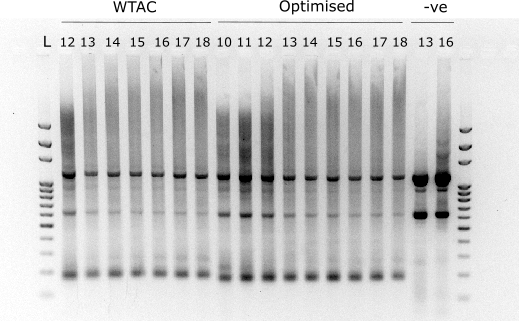
\includegraphics[width=\linewidth, height=0.15\textheight]{Figures/WTAC_Adapted_Gel1.png}
		\caption{Gel image of WTAC and optimised protocol}
	\end{subfigure}
	\hspace{2em}
	\begin{subfigure}{0.4\linewidth}
		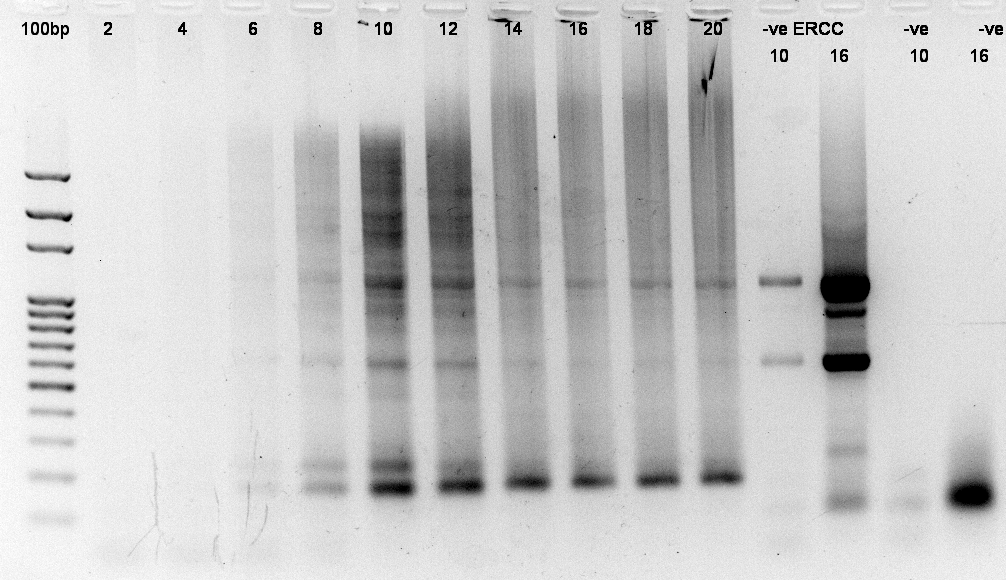
\includegraphics[width=\linewidth, height=0.15\textheight]{Figures/WTAC_Adapted_Final.png}
		\caption{Gel image from repeat of optimised protocol}
	\end{subfigure}
	\captionsetup{width=0.95\textwidth}
	\caption[Gel image of repeated optimised protocol]%
	{\textbf{Gel images of WTAC and optimised protocol for SMART-seq2 cDNA synthesis}: Figure a) Amplified DNA from original WTAC and optimised protocol taken from cycles 12 to 18 were run on 1\% agarose gel. Figure b) Repeated optimised protocol with a greater range of cycles and lower ERCC RNA spike-in concentration. Numbers represent the number of cycles, L refers to 100bp ladder. -ve refers to negative control with water.} 
	\label{fig:wtac_optimised_gel1_2}
\end{figure} 
\resumetocwriting
